\documentclass[UTF-8]{ctexart}
\usepackage{geometry}
\usepackage{graphicx}
\usepackage[namelimits]{amsmath} %数学公式
\usepackage{amssymb}             %数学公式             %数学字体
\usepackage{mathrsfs} 
\usepackage{txfonts}
\usepackage{float}  %设置图片浮动位置的宏包
\usepackage{subfigure}%插入多图时用子图显示的宏包
\geometry{a4paper,scale=0.85}
\author{左熙辰\thanks{北京大学生命科学学院;e-mail:m13333318502@163.com}}
\date{}
\title{麻醉剂和酒精对斑马鱼幼体的影响}
\begin{document}
    \maketitle
    \begin{abstract}
        斑马鱼是一种实验室常见的小型脊椎动物,因其发育过程较为简单,卵透明便于观察发育全过程而受到科学家青睐,本文将使用野生型斑马鱼探究麻醉剂和乙醇对斑马鱼幼体心率的影响。
    \end{abstract}
    \paragraph*{关键字}斑马鱼\text{ }发育生物学\text{ } 心率 
    \section{实验方法}
    取一培养皿健康的幼体斑马鱼,统计心率,再施以麻醉剂(三卡因,Tricanie),待其完全麻醉后,统计心率并移除麻醉剂,恢复后重新统计心率,然后加入5\%的乙醇溶液,统计心率并迅速转移,恢复后再次测定斑马鱼心率
    \section{实验结果及结论}
    实验结果如下图所示,三卡因处理后和移除后,心源性活动并未受到抑制,所以心率基本不变,而乙醇处理后,心肌细胞受到乙醇毒害,心率活动受到一定的抑制但结果并不显著,乙醇移除后,心率逐步恢复。
    \begin{figure}[h]
        \centering
        \subfigure[]{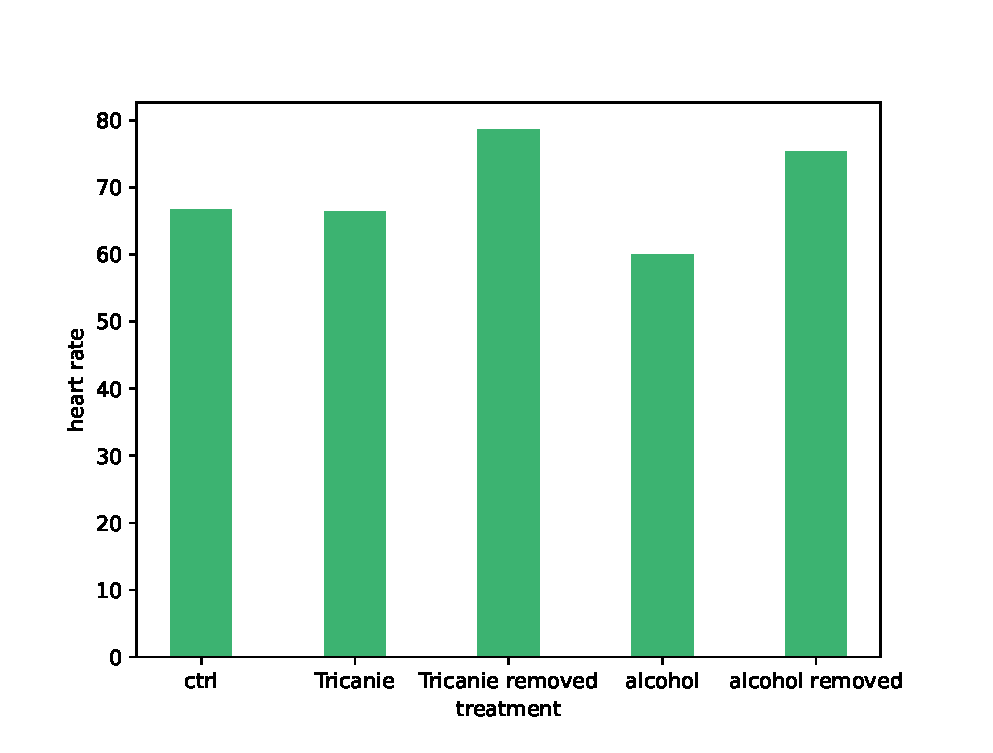
\includegraphics[scale = 0.5]{src/zoology/Figure1.eps}}
        \subfigure[]{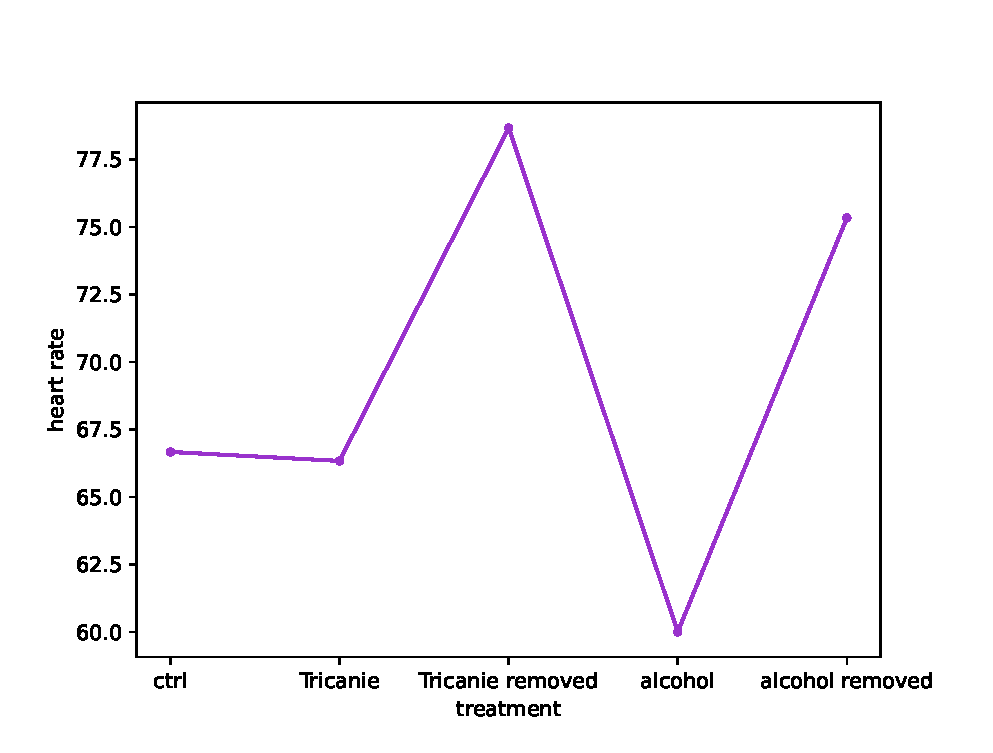
\includegraphics[scale = 0.5]{src/zoology/Figure2.eps}}
        \caption[]{\textbf{不同处理对斑马鱼幼体心率的影响.}其中ctrl为处理前对照,Tricanie为三卡因处理组,Tricanie removed为三卡因移除组,
        Alcohol为乙醇处理组,Alchol removed为乙醇移除组,ctrl组与Tricine组采用Student's-t检验,剩下相邻两组进行Kolmogorov-Smirnov检验,五组均无显著差异(\textit{P}=0.91, 0.09, 0.09, 0.6, 0.6; \textit{P}>0.05)}
    \end{figure}

\end{document}